% Enable warnings about problematic code
\RequirePackage[l2tabu, orthodox]{nag}

\documentclass{WeSTassignment}

% The lecture title, e.g. "Web Information Retrieval".
\lecture{Introduction to Web Science}
% The names of the lecturer and the instructor(s)
\author{%
  Prof. Dr.~Steffen~Staab\\{\normalsize\mailto{staab@uni-koblenz.de}} \and
  Ren{\'e}~Pickhardt\\{\normalsize\mailto{rpickhardt@uni-koblenz.de}} \and
   Korok~Sengupta\\{\normalsize\mailto{koroksengupta@uni-koblenz.de}}
}
% Assignment number.
\assignmentnumber{2}
% Institute of lecture.
\institute{%
  Institute of Web Science and Technologies\\%
  Department of Computer Science\\%
  University of Koblenz-Landau%
}
% Date until students should submit their solutions.
\datesubmission{November 9, 2016, 10:00 a.m.}
% Date on which the assignments will be discussed in the tutorial.
\datetutorial{November 11th, 2016, 12:00 p.m.}

% Set langauge of text.
\setdefaultlanguage[
  variant = american, % Use American instead of Britsh English.
]{english}

% Specify bib file location.
\addbibresource{bibliography.bib}

% For left aligned centerd boxes
% see http://tex.stackexchange.com/a/25591/75225
\usepackage{varwidth}

% ==============================================================================
% Document

\begin{document}

\maketitle

The main objective of this assignment is for you to use different tools with which you can understand the network that you are connected to or you are connecting to in a better sense.
These tasks are not always specific to \enquote{Introduction to Web Science}.
For all the assignment questions that require you to write a code, make sure to include the code in the answer sheet, along with a separate python file. Where screen shots are required, please add them in the answers directly and not as separate files. 

Team: \textbf{Papa}
\\Team members:
\begin{enumerate}
\item Brigitte Aznar
\item Bonasmitha Behura
\item Ilia Tugushi
\end{enumerate}
% ------------------------------------------------------------------------------

\section{IP Packet (5 Points)}

Consider the IPv4 packet that is received as:\\ \\
\texttt{4500 062A 42A1 8001 4210 XXXX C0A8 0001 C0A8 0003}\\ \\ 
Consider \texttt{XXXX} to be the check sum field that needs to be sent with the packet.

Please provide a step-by-step process for calculating the "Check Sum".\\ \\ 

\begin{enumerate}
\item Calculating the sum of the header \\
4500 + 062A + 42A1 + 8001 + 4210 + C0A8 + 0001 + C0A8 + 0003 = \textbf{2D130}
\item Transform the result into binary\\
0010 1101 0001 0011 0000
\item Add the first 4 bits to the rest of the value\\
0010 + 1101 0001 0011 0000 = \textbf{1101 0001 0011 0010}
\item Flip the 1s and 0s to get the check sum\\
1101  0001  0011  0010\\
\textbf{0010 1110 1100 1101}
\item Transform the previous result back into hex\\
The check sum is \textbf{2ECD}
\end{enumerate}

% ------------------------------------------------------------------------------

\section{Routing Algorithm (10 Points)}
\textbf{UPDATE. The bold fonted numbers have been updated on Monday Nov. 7th. (If you already have done so feel free to use the old numbers. But the solution with the old version will be more complex than the solution with the updated numbers.)}

You have seen how routing tables can be used to see how the packets are transferred across different networks. Using the routing tables below of Router 1, 2 and 3:
\begin{enumerate}
\item Draw the network \texttt{[6 points]}
\item Find the shortest path of sending information from 67.68.2.10 network to 25.30.3.13 network \texttt{[4 points]}
\end{enumerate}

\begin{table}[h]
\centering
\caption{Router 1}
\label{Router 1}
\begin{tabular}{ccc}
\hline
\multicolumn{1}{|c|}{\textbf{Destination}} & \multicolumn{1}{c|}{\textbf{Next Hop}} & \multicolumn{1}{c|}{\textbf{Interface}} \\ \hline
67.0.0.0                                   & 67.68.3.1                              & eth 0                                   \\
62.0.0.0                                   & 62.4.31.7                              & eth 1                                   \\
88.0.0.0                                   & 88.4.32.6                              & eth 2                                    \\
141.\textbf{71}.0.0                                  & 141.\textbf{71}.20.1                            & eth 3                                    \\
26.0.0.0                                   & 141.71.26.3                            & eth 3                                   \\
\textbf{156.3}.0.0                                  & 141.71.26.3                            & eth 3                                   \\
205.\textbf{30.7}.0                                  & 141.71.26.3                            & eth 3                                    \\
25.0.0.0                                   & 88.6.32.1                              & eth 2                                    \\
121.0.0.0                                  & 88.6.32.1                              & eth 2                                   
\end{tabular}
\end{table}
\begin{table}[h]
\centering
\caption{Router 2}
\label{Router 2}
\begin{tabular}{ccc}
\hline
\multicolumn{1}{|c|}{\textbf{Destination}} & \multicolumn{1}{c|}{\textbf{Next Hop}} & \multicolumn{1}{c|}{\textbf{Interface}} \\ \hline
141.\textbf{71}.0.0                                  & 141.71.26.3                            & eth 3                                   \\
205.\textbf{30.7}.0                                  & 205.\textbf{30.7}.1                            & eth 0                                   \\
26.0.0.0                                   & 26.3.2.1                               & eth 2                                    \\
156.\textbf{3}.0.0                                  & 156.3.0.6                              & eth 1                                   \\
67.0.0.0                                   & 141.\textbf{71}.20.1                            & eth 3                                   \\
62.0.0.0                                   & 141.\textbf{71}.20.1                            & eth 3                                   \\
88.0.0.0                                   & 141.\textbf{71}.20.1                            & eth 3                                    \\
25.0.0.0                                   & 205.30.7.2                             & eth 0                                   \\
121.0.0.0                                  & 205.30.7.2                             & eth 0                                  
\end{tabular}
\end{table}
\begin{table}[!ht]
\centering
\caption{Router 3}
\label{Router 3}
\begin{tabular}{ccc}
\hline
\multicolumn{1}{|c|}{\textbf{Destination}} & \multicolumn{1}{c|}{\textbf{Next Hop}} & \multicolumn{1}{c|}{\textbf{Interface}} \\ \hline
205.\textbf{30.7}.0                                  & 205.30.7.2                             & eth 0                                   \\
88.0.0.0                                   & 88.6.32.1                              & eth 1                                   \\
25.0.0.0                                   & 25.30.1.2                              & eth 2                                   \\
121.0.0.0                                  & 121.0.3.1                              & eth 3                                   \\
156.\textbf{3}.0.0                                  & 205.\textbf{30}.7.1                             & eth 0                                   \\
26.0.0.0                                   & 205.\textbf{30}.7.1                             & eth 0                                   \\
141.0.0.0                                  & 205.\textbf{30}.7.1                             & eth 0                                   \\
67.0.0.0                                   & 88.4.32.6                              & eth 1                                   \\
62.0.0.0                                   & 88.4.32.6                              & eth 1                                  
\end{tabular}
\end{table}
\clearpage
\begin{enumerate}
\item
	\begin{figure}[!hb]
  	\centering
  	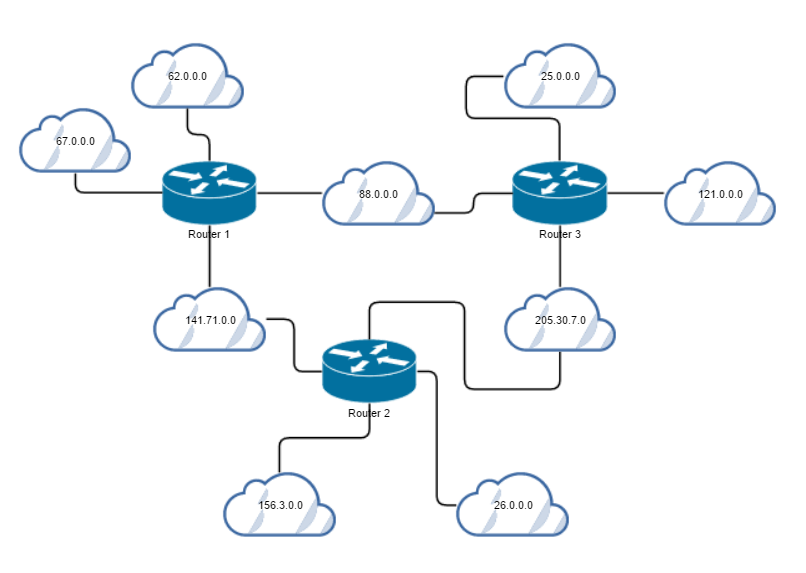
\includegraphics[width=0.9\textwidth]{network_diagram.png}
   	\caption{Network diagram}
     \label{fig:network diagram}
	\end{figure}
\item 
	\begin{enumerate}
	\item Goes from 67.0.0.0 network to Router 1
	\item Gets out of Router 1 through eth2 to the 88.0.0.0 network
	\item Gets into Router 3 trough eth 1
	\item Finally it's sent to the 25.0.0.0 network through eth2 and finds 25.30.3.13
	\end{enumerate}
\end{enumerate}

% ------------------------------------------------------------------------------


\section{Sliding Window Protocol (10 Points)}
\emph{Sliding window algorithm, which allows a sender to have more than one unacknowledged packet "in flight" at a time, improves network throughput. }\\ \\
Let us consider you have 2 Wide Area Networks. One with a bandwidth of 10 Mbps (Delay of 20 ms) and the other with 1 Mbps (Delay of 30 ms) . If a packet is considered to be of size 10kb. Calculate the window size of number of packets necessary for Sliding Window Protocol. [\texttt{5 points}]\\ \\
\\ \\
\[p   = 10kb\]\\
\[D_1= 20ms = 0.02s\]\\
\[B_1 = 10Mbps\]\\
\[D_2= 30ms = 0.03s\]\\
\[B_2 = 1Mbps\]\\
\[W = 2*B*D\]\\
\[W = 2 * 10Mb/s * 0.02s = 0.40Mb = 400Kb\]\\
\[WP = 400kb / 10kb = 40 packages\]\\
\[W = 2 * 1Mb/s * 0.03s = 0.06Mb = 60Kb\]\\
\[WP = 60kb / 10kb = \textbf{6 packages}\] \\

Since the sliding window protocol is made for avoiding overflowing from one fast network to a slower one we would then take the smallest package size for them to communicate.\\

** being W the window size in Kb\\ WP the number of packages per window\\ B the bandwidth\\ D delay\\\\
Since you now understand the concept of Window Size for Sliding Window Protocol and how to calculate it, consider a window size of 3 packets and you have 7 packets to send. Draw the process of \texttt{Selective Repeat Sliding Window Protocol} where in the 3rd packet from the sender is lost while transmission. Show diagrammatically how the system reacts when a packet is not received and how it recuperates from that scenario. [\texttt{5 points}] \\




% ------------------------------------------------------------------------------

\section{TCP Client Server (10 Points)}

Use the information from the \href{https://docs.python.org/3/howto/sockets.html}{socket} documentation and create: [\texttt{4 points}]
\begin{enumerate}
\item a simple TCP Server that listens to a
\item Client
\end{enumerate}
\underline{Note:} Please use port \texttt{8080} for communication on \texttt{localhost} for client server communication.\\ \\
Given below are the following points that your client and server must perform: [\texttt{6 points}]
\begin{enumerate}
\item The \emph{Client} side asks the user to input their name, age \& \emph{matrikelnummer} which is then sent to the server all together.
\item Develop a protocol for sending these three information and subsequently receiving each of the information in three different lines as mentioned in the below format. Provide reasons for the protocol you implemented. 
\item Format the output in a readable format as:\texttt{\\ Name: Korok Sengupta; \\ Age: 29; \\ Matrikelnummer: 21223ert56}
\end{enumerate}

Provide a snapshot of the results along with the code. \\


For the server side:
\begin{lstlisting}
#papa_assignment2_4_server.py
import socket
import json

def Main():

    socket_server = socket.socket()
    socket_server.bind(('localhost', 8080))

    socket_server.listen(1)
    conn, addr = socket_server.accept()
    print("Connection from: " + str(addr))
    data = conn.recv(1024)
    data = data.decode('utf-8')
    if not data:
        print('no data received')
        return

    data = json.loads(data)
    message = 'Name: {}\nAge: {}\nMatrikelnummer: {}'.format(data['name'], data['age'], data['matrikel'])
    print(message)

    conn.close()


if __name__ == '__main__':
    Main()
\end{lstlisting}

For the client side:
\begin{lstlisting}
#papa_assignment2_4_client.py
import socket
import json 
def Main():
    host = 'localhost'
    port = 8080

    name     = input('Enter your name: ')
    age      = input('Enter your age: ')
    m_nummer = input('Enter your matrikelnummer: ')

    clientSocket = socket.socket()
    clientSocket.connect((host, port))

    data = {}
    data['name'] = name
    data['age'] = age
    data['matrikel'] = m_nummer
    json_data = json.dumps(data)
    clientSocket.send(json_data.encode('utf-8'))

    clientSocket.close()


if __name__ == '__main__':
    Main()
\end{lstlisting}
\begin{figure}[h]
  	\centering
  	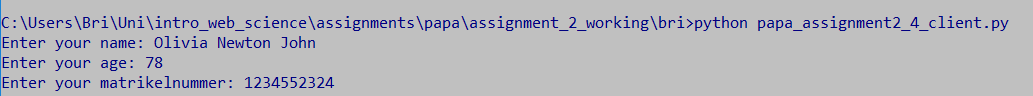
\includegraphics[width=0.9\textwidth]{results_client.png}
   	\caption{Client results}
     \label{fig:client}
\end{figure}
\begin{figure}[h]
  	\centering
  	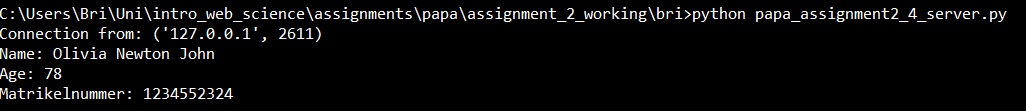
\includegraphics[width=0.9\textwidth]{results_server.png}
   	\caption{Server results}
     \label{fig:server}
\end{figure}


We used this json because is a very clean way to send and receive data it is also safe to decode/encode.
\makefooter

\end{document}
